\documentclass[11pt,a4paper]{article}
\usepackage[margin=20mm,top=18mm,bottom=19mm]{geometry}
\usepackage{graphicx,booktabs,xcolor,hyperref}
\definecolor{ink}{HTML}{172C3C}
\definecolor{accent}{HTML}{26687A}
\definecolor{ruleblue}{HTML}{D5E2E6}
\hypersetup{colorlinks=true,linkcolor=accent,urlcolor=accent,citecolor=accent,
  pdftitle={CS 464 Progress Report -- ZooLake Plankton Classification}}
\setlength{\parindent}{0pt}
\setlength{\parskip}{5pt plus 1pt}
\setlength{\abovecaptionskip}{3pt}
\setlength{\belowcaptionskip}{1pt}
\renewcommand{\arraystretch}{1.14}
\newcommand{\masthead}[1]{%
  {\small\sffamily\bfseries\color{accent} BILKENT UNIVERSITY \enspace / \enspace CS 464 MACHINE LEARNING}
  \hfill{\small\sffamily\color{accent} #1}\par
  \noindent{\color{ruleblue}\rule{\linewidth}{0.7pt}}\vspace{4pt}\par}
\newcommand{\sectiontitle}[1]{\vspace{4pt}{\large\sffamily\bfseries\color{ink}#1}\par}
\newcommand{\subheading}[1]{{\sffamily\bfseries\color{accent}#1}\par}
\newcommand{\figureline}[2]{{\small\sffamily\textbf{Figure #1.} #2}\par}
\raggedbottom

\begin{document}
\color{ink}
\masthead{PROJECT PROGRESS REPORT}
\vspace{4mm}
{\huge\bfseries\raggedright Sample-Efficient and Rotation-Robust\\
Plankton Image Classification on ZooLake\par}
\vspace{2mm}
{\small\sffamily
\begin{tabular}{@{}l@{\quad}r@{\hspace{10mm}}l@{\quad}r@{}}
Kerem Emre Bayrak & 22303713 & Deniz Can Yoldaş & 22303392 \\
Mehmet Mert Suci & 22303444 & Osman Kaan Kasap & 21902345
\end{tabular}\hfill 20 November 2026\par}
\vspace{2mm}

\sectiontitle{1 \quad Introduction}
Plankton can appear at many orientations in a microscope image, and rare categories may have only a handful of labels. We study how much labeled data a classifier needs and whether training on rotations and reflections improves performance. ZooLake is the current dataset following reported TA feedback on the submitted Galaxy10 DECaLS proposal. Whether the final deliverable should also include a Galaxy10 comparison remains open.

The first milestone establishes a reproducible split and a CPU baseline. We use macro-F1 as the primary metric so that every label has equal weight. We also report accuracy and the mean F1 of the least represented training classes.

\sectiontitle{2 \quad Dataset}
\subheading{2.1 \quad Dataset analysis}
ZooLake consists of dark-background regions of interest extracted from lower-magnification images of Lake Greifensee, Switzerland, captured by the Dual Scripps Plankton Camera~\cite{zoolake}. The 35 labels include zooplankton taxa, colonial phytoplankton, and categories such as debris, skins, and unknown objects. The Eawag release provides one image directory per label, feature sidecars and provider fold lists~\cite{archive}.

All 17,943 files decoded as RGB JPEGs. The alphabetical folder order matched the 35-entry provider class array. Width ranged from 16 to 2,832 pixels (median 72) and height from 20 to 2,176 pixels (median 76). The most frequent label, \textit{dinobryon}, has 3,321 images, while \textit{chaoborus} has 10, a ratio of 332 to 1. Three exact pixel-duplicate pairs had conflicting labels.

\begin{center}
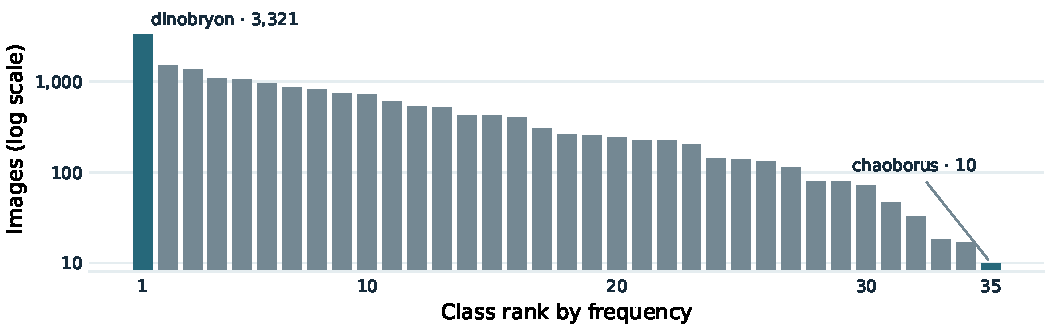
\includegraphics[width=\linewidth]{class_distribution.pdf}
\end{center}
\figureline{1}{Class sizes in the downloaded archive, before quarantine. A logarithmic count axis makes rare classes visible.}

\newpage
\masthead{DATA AND METHODS}
\sectiontitle{2 \quad Dataset \textnormal{\small (continued)}}
\subheading{2.2 \quad Dataset preprocessing}
The provider lists repeated two image paths across folds. Even after quarantining both files in each conflicting duplicate pair, 1,487 capture-block components crossed the provider boundaries. We generated a new grouped split using seed 464. Grouping by UTC day, hour, or ten-minute block could place \texttt{maybe\_cyano} in at most two folds. Five-minute grouping left only 11 examples in its smallest block. Three-minute UTC blocks gave it supports of 975, 225, and 164 and allowed all 35 labels to appear in each fold. Capture times were read from the original ROI filenames~\cite{eyring}.

\begin{center}
\small
\begin{tabular}{@{}lrrr@{}}
\toprule
Partition & Images & Capture blocks & Smallest class \\
\midrule
Train & 12,556 & 4,964 & 5 \\
Validation & 2,690 & 572 & 1 \\
Final test & 2,691 & 626 & 2 \\
\bottomrule
\end{tabular}
\end{center}

The 17,937 retained images give an approximately stratified 70/15/15 split. Exact decoded duplicates, frames, and three-minute blocks stay within a single fold. Longer acquisition sessions and visually similar crops can still span folds. For example, a large \textit{asterionella} block also skewed its validation support to 48 out of 1,054 retained images.

Oversized crops were shrunk to fit a $128 \times 128$ canvas, preserving aspect ratio. Black padding centered the crop. Feature extraction was fixed, and standardization parameters were fitted on training images only. The run used one view per image throughout.

\sectiontitle{3 \quad Coding environment}
We used Python 3.13.3, Pillow 11.2.1, NumPy 2.2.5, SciPy 1.17.0, scikit-learn 1.8.0, and Matplotlib 3.10.1. The baseline ran on an Apple M2 Pro with 10 CPU cores and 32 GB of unified memory. PyTorch 2.10.0 and torchvision 0.25.0 support the CNN experiments. Metal was verified in a native process. The project CLI saves audit and split manifests, configuration, a fitted model, and validation predictions.

\sectiontitle{4 \quad Details of the trained model}
The trained baseline was L2-regularized multinomial logistic regression. Each image produced 104 features from a coarse grayscale grid, foreground color histograms and moments, simple foreground geometry, and horizontal and vertical edge statistics. The model learns one linear score per class and converts the scores to probabilities with softmax. We used inverse-frequency class weights and $C=1$. Decreasing $C$ increases regularization. Class weighting makes rare examples matter more to the loss and can reduce precision if the model overpredicts rare categories.

\sectiontitle{5 \quad Experimental setup}
The progress run used the full training fold, seed 464 and a single validation pass. The final test fold stays sealed until the experiment settings are chosen. For the learning curve, each of seeds 464--466 has nested 10/25/50/100\% subsets with 1,256, 3,139, 6,278 and 12,556 images. At 10\%, proportional allocation would give \textit{chaoborus} half an image. Reserving one image per class before allocating the remaining budget preserves all labels and keeps the global subset size fixed.

\newpage
\masthead{VALIDATION AND NEXT MILESTONES}
\sectiontitle{6 \quad Results}
\begin{center}
\small
\begin{tabular}{@{}lrrr@{}}
\toprule
Single-view validation ($n=2{,}690$) & Macro-F1 & Minority macro-F1 & Accuracy \\
\midrule
Weighted logistic regression & \textbf{0.512} & 0.145 & 69.37\% \\
\bottomrule
\end{tabular}
\end{center}

The minority group includes the nine labels with the lowest training support. \textit{Dinobryon} scored 0.776 on 595 examples. The model missed all 3 \textit{chaoborus}, 4 \textit{diatom\_chain}, and 1 \textit{hydra} examples, so a single image can change these estimates substantially. Feature extraction, fitting, and prediction took about 11 seconds on CPU.

\begin{center}
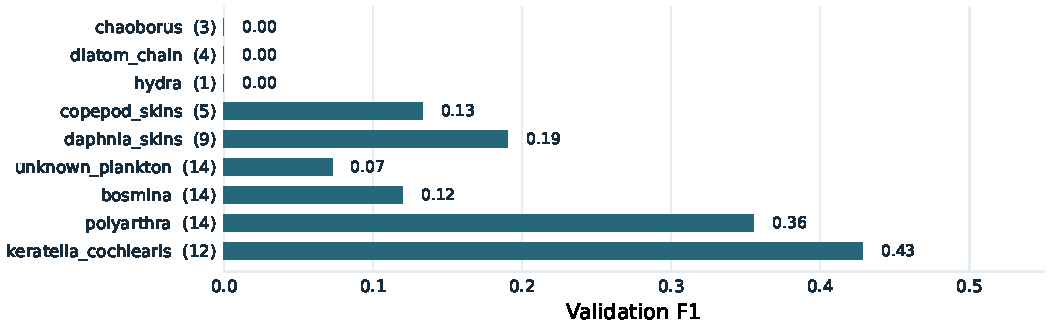
\includegraphics[width=\linewidth]{minority_f1.pdf}
\end{center}
\figureline{2}{Minority-class validation F1. Numbers in parentheses are the validation support for each label.}

Next, we will compare no augmentation with D4 training on matched subsets for a scratch CNN and ImageNet-pretrained EfficientNet-B0~\cite{efficientnet}. On each checkpoint, we will compare one view with mean probabilities over eight D4 views. Synthetic batches project roughly 1 and 55 minutes per full-budget CPU epoch, respectively. A GPU pilot will inform the three-seed schedule.

\sectiontitle{7 \quad Workload distribution}
The following responsibilities cover verification of the progress results and the next experiments.

{\small\setlength{\tabcolsep}{5pt}
\begin{tabular}{@{}p{37mm}p{124mm}@{}}
\toprule
\textbf{Member} & \textbf{Responsibility} \\
\midrule
Mehmet Mert Suci & Reproduce the data audit and split. Check duplicate cases and explain how the 10\% subset keeps all labels. \\
Kerem Emre Bayrak & Reproduce the handcrafted-feature baseline. Verify training-only scaling and review the largest classification errors. \\
Deniz Can Yoldaş & Run the scratch CNN pilots. Compare D4 augmentation and one-view versus eight-view inference on validation. \\
Osman Kaan Kasap & Time the EfficientNet-B0 pilot. Set feasible training budgets and prepare the learning curves and minority-class comparisons. \\
\bottomrule
\end{tabular}
\par}

\vspace{-2pt}
{\small
\renewcommand{\refname}{\large\sffamily References}
\begin{thebibliography}{9}
\setlength{\itemsep}{1pt}
\bibitem{zoolake} S.\ P. Kyathanahally et al. Deep Learning Classification of Lake Zooplankton. \textit{Frontiers in Microbiology} 12, 746297, 2021. \href{https://doi.org/10.3389/fmicb.2021.746297}{doi:10.3389/fmicb.2021.746297}.
\bibitem{archive} Eawag. \textit{Deep Learning Classification of Zooplankton from Lakes}, ZooLake release. \href{https://opendata.eawag.ch/dataset/52b6ba86-5ecb-448c-8c01-eec7cb209dc7}{Eawag Open Data}.
\bibitem{eyring} S.\ Eyring et al. Five years of high-frequency data of phytoplankton zooplankton and limnology from a temperate eutrophic lake. \textit{Scientific Data} 12, 653, 2025. \href{https://doi.org/10.1038/s41597-025-04988-9}{doi:10.1038/s41597-025-04988-9}.
\bibitem{efficientnet} M.\ Tan and Q.\ Le. EfficientNet: Rethinking Model Scaling for Convolutional Neural Networks. \textit{ICML}, 2019. \href{https://proceedings.mlr.press/v97/tan19a.html}{PMLR 97, 6105--6114}.
\end{thebibliography}
}
\end{document}
